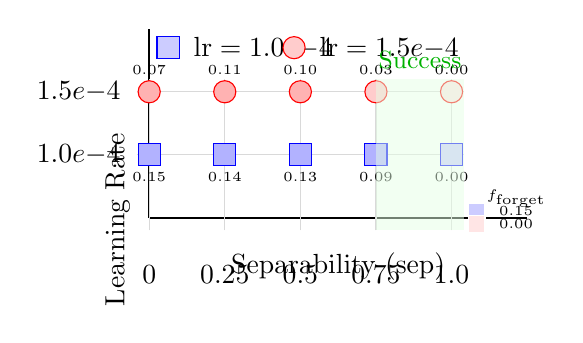
\begin{tikzpicture}[scale=0.8]
  % Axes
  \draw[thick] (0,0) -- (6,0);
  \draw[thick] (0,0) -- (0,3);

  \node[below] at (3,-0.4) {Separability ($\mathrm{sep}$)};
  \node[left,rotate=90] at (-0.5,1.5) {Learning Rate};

  % X-axis: sep (0 to 1)
  \node[below] at (0,-0.6) {0};
  \node[below] at (1.2,-0.6) {0.25};
  \node[below] at (2.4,-0.6) {0.5};
  \node[below] at (3.6,-0.6) {0.75};
  \node[below] at (4.8,-0.6) {1.0};

  % Y-axis: lr
  \node[left] at (-0.3,1.0) {$1.0e\text{-}4$};
  \node[left] at (-0.3,2.0) {$1.5e\text{-}4$};

  % Horizontal lines for lr values
  \draw[gray!30] (-0.2,1.0) -- (5.0,1.0);
  \draw[gray!30] (-0.2,2.0) -- (5.0,2.0);

  % Vertical lines for sep values
  \foreach \x in {0,1.2,2.4,3.6,4.8} \draw[gray!30] (\x,-0.2) -- (\x,2.2);

  % Data points for lr=1e-4 (blue squares)
  % sep=0: 0.146, sep=0.25: 0.136, sep=0.5: 0.132, sep=0.75: 0.091, sep=1.0: 0.002
  \node[draw=blue, fill=blue!30, rectangle, minimum size=8pt, inner sep=0pt] at (0,1) {};
  \node[draw=blue, fill=blue!30, rectangle, minimum size=8pt, inner sep=0pt] at (1.2,1) {};
  \node[draw=blue, fill=blue!30, rectangle, minimum size=8pt, inner sep=0pt] at (2.4,1) {};
  \node[draw=blue, fill=blue!30, rectangle, minimum size=8pt, inner sep=0pt] at (3.6,1) {};
  \node[draw=blue, fill=blue!20, rectangle, minimum size=8pt, inner sep=0pt] at (4.8,1) {};

  % Value labels for lr=1e-4
  \node[font=\tiny] at (0,0.65) {0.15};
  \node[font=\tiny] at (1.2,0.65) {0.14};
  \node[font=\tiny] at (2.4,0.65) {0.13};
  \node[font=\tiny] at (3.6,0.65) {0.09};
  \node[font=\tiny] at (4.8,0.65) {0.00};

  % Data points for lr=1.5e-4 (red circles)
  % sep=0: 0.071, sep=0.25: 0.111, sep=0.5: 0.099, sep=0.75: 0.028, sep=1.0: 0.000
  \node[draw=red, fill=red!30, circle, minimum size=8pt, inner sep=0pt] at (0,2) {};
  \node[draw=red, fill=red!30, circle, minimum size=8pt, inner sep=0pt] at (1.2,2) {};
  \node[draw=red, fill=red!30, circle, minimum size=8pt, inner sep=0pt] at (2.4,2) {};
  \node[draw=red, fill=red!20, circle, minimum size=8pt, inner sep=0pt] at (3.6,2) {};
  \node[draw=red, fill=red!10, circle, minimum size=8pt, inner sep=0pt] at (4.8,2) {};

  % Value labels for lr=1.5e-4
  \node[font=\tiny] at (0,2.35) {0.07};
  \node[font=\tiny] at (1.2,2.35) {0.11};
  \node[font=\tiny] at (2.4,2.35) {0.10};
  \node[font=\tiny] at (3.6,2.35) {0.03};
  \node[font=\tiny] at (4.8,2.35) {0.00};

  % Legend
  \node[draw=blue, fill=blue!20, rectangle, minimum size=8pt, inner sep=0pt] at (0.3,2.7) {};
  \node[right] at (0.55,2.7) {$\mathrm{lr}=1.0e\text{-}4$};

  \node[draw=red, fill=red!20, circle, minimum size=8pt, inner sep=0pt] at (2.3,2.7) {};
  \node[right] at (2.55,2.7) {$\mathrm{lr}=1.5e\text{-}4$};

  % Success region shading
  \fill[green!10, opacity=0.5] (3.6,-0.2) rectangle (5.0,2.2);
  \node[green!70!black, font=\small] at (4.3,2.5) {Success};

  % Color scale indicator
  \node[font=\tiny, right] at (5.2,0.3) {$f_{\mathrm{forget}}$};
  \node[draw=white, fill=blue!20, rectangle, minimum size=6pt, inner sep=0pt] at (5.2,0.1) {};
  \node[font=\tiny, right] at (5.4,0.1) {0.15};

  \node[draw=white, fill=red!10, rectangle, minimum size=6pt, inner sep=0pt] at (5.2,-0.1) {};
  \node[font=\tiny, right] at (5.4,-0.1) {0.00};
\end{tikzpicture}
